\section{Flyback Converter Design}

\begin{figure}[H]
\begin{center}
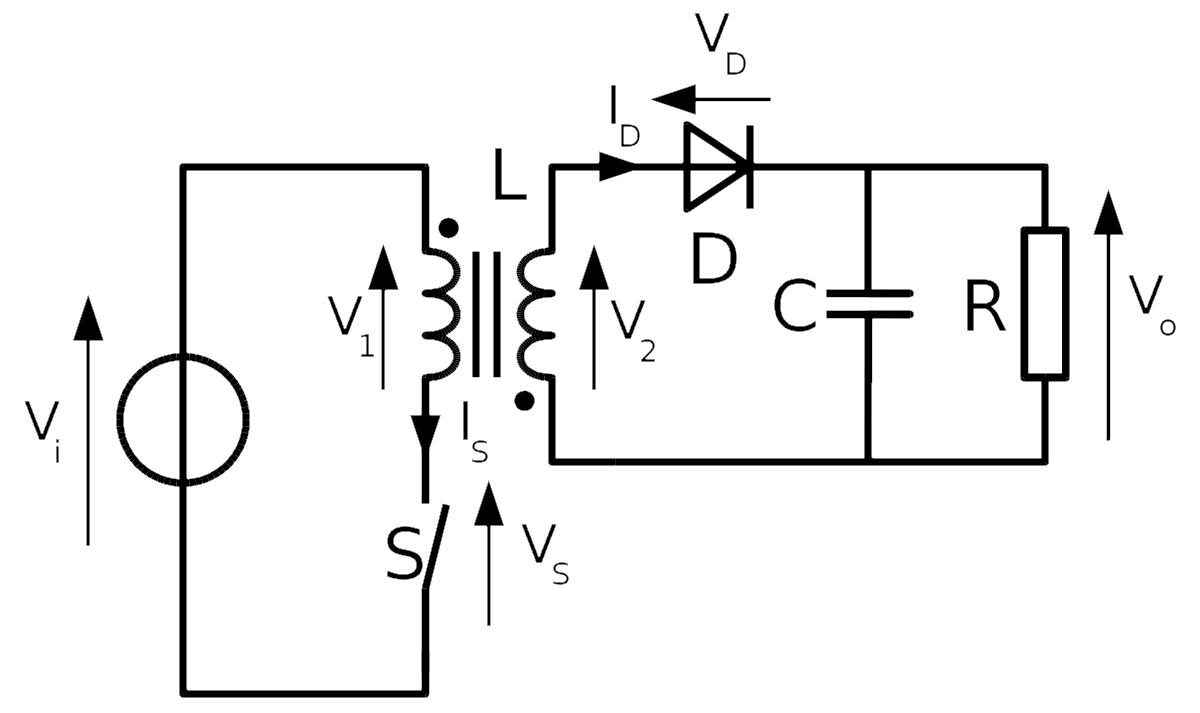
\includegraphics[width=0.6\textwidth]{figures/flybacktop.png}
\caption{Ideal Flyback Converter}
\label{fig:flybacktop}
\end{center}
\end{figure}

The general circuit schematic of an ideal flyback converter topology is given in Figure \ref{fig:flybacktop}. It is a galvanically isolated DC-DC converter with a special feature. That special feature is using the magnetizing inductance of the transformer as an energy storage device, instead of a separate circuit component, which helps reduce the cost, volume and mass of the converter. For our hardware project, we will build a Flyback Converter with extra features to establish the flexibility and performance required to achieve the main requirements and collect bonus points from the Hardware Project. 
\par Our circuit's main controller is UCC28740 by Texas Instruments. It can achieve both current mode and voltage mode control by taking feedback from input and output sides of the converter. For UCC28740 to perform properly, the rest of the circuit should be set to achieve DCM operation at all times. UCC28740 can achieve valley switching, which means it will try to switch the MOSFET at the lowest possible voltage than the primary voltage to reduce the switching losses, and hence increase the efficiency. Those voltage levels are called valley points which are bottoms of the voltage swing at the primary side of the transformer, as seen in Figure \ref{fig:valleyswitch}. The lower voltage level is seen because of the ringing when primary current reaches zero. This kind of Flyback Converter is called Quasi-Resonant Flyback Converter. The selected UCC28740 controller is able to realize this operation mode for the Flyback Converter so that the switching losses are reduced, and hence the efficiency is increased. This operation will also reduce the cooling requirements of the switching device since its switching losses are reduced, which results in smaller sized cooling equipments like heat sinks.

\begin{figure}[H]
\begin{center}
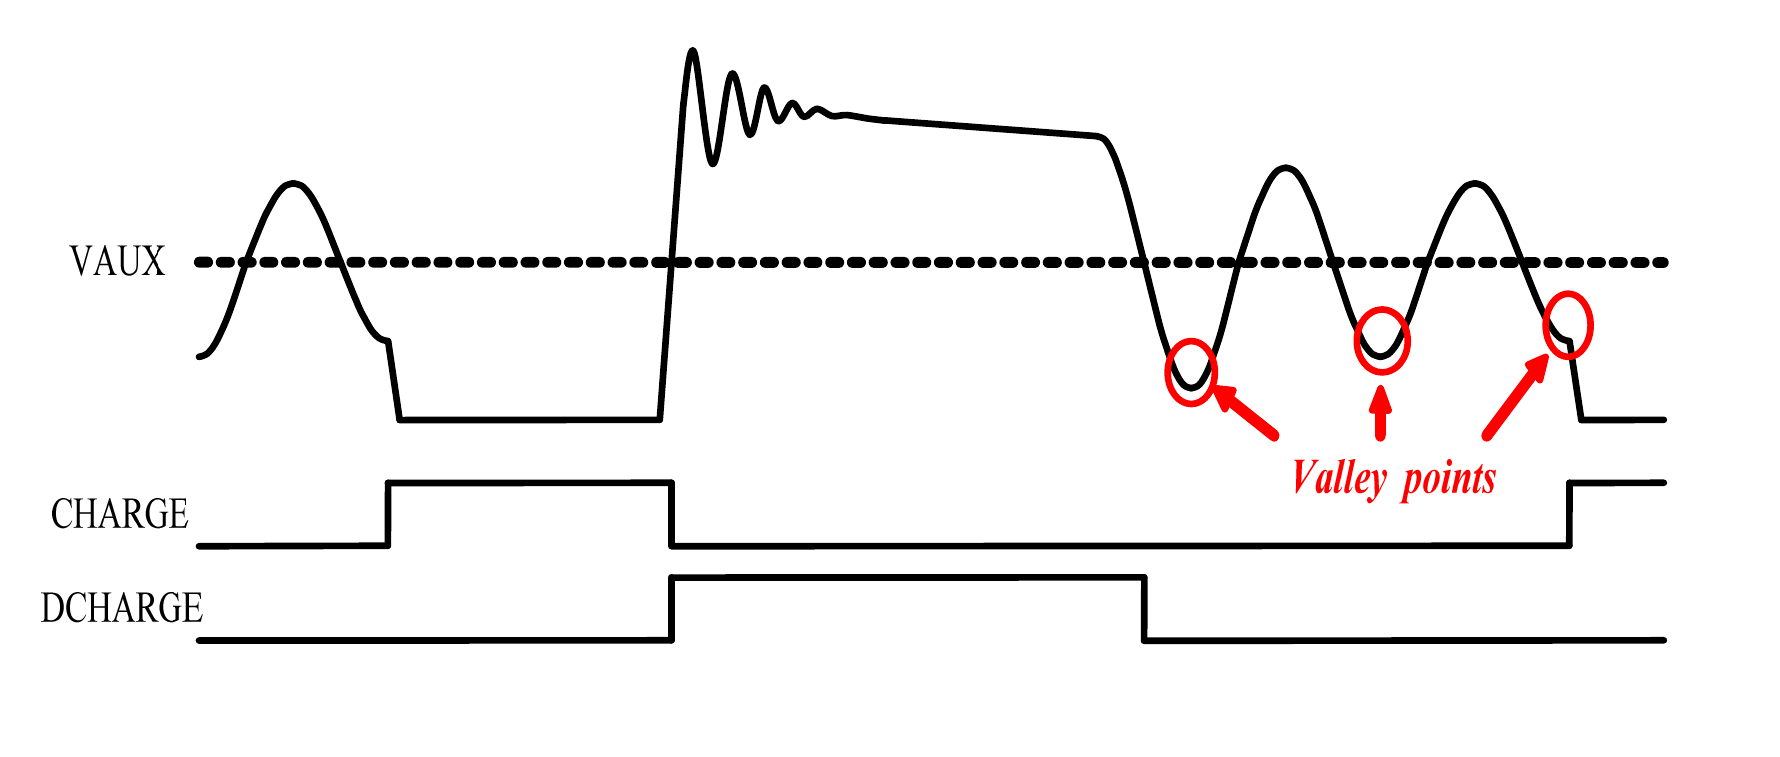
\includegraphics[width=0.6\textwidth]{figures/valleyswitch.png}
\caption{Vallet Points of a Quasi-Resonant Flyback Converter}
\label{fig:valleyswitch}
\end{center}
\end{figure}

The reference design for the mentioned IC is given in Figure \ref{fig:refdesign}.

\begin{figure}[H]
\begin{center}
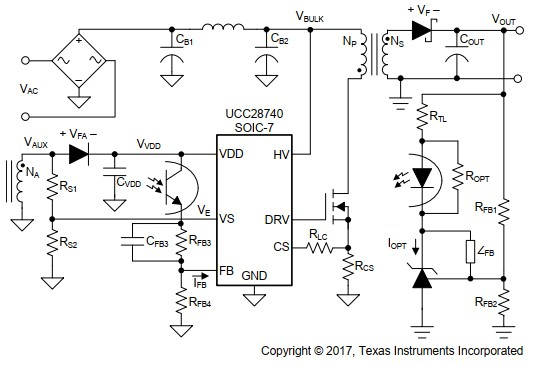
\includegraphics[width=0.8\textwidth]{figures/refdesign.jpg}
\caption{Reference Flyback Converter Design with UCC28740}
\label{fig:refdesign}
\end{center}
\end{figure}

Since our input voltage is directly going to be an adjustable DC voltage, we do not require the bridge rectifier and the rectifier output filter and the EMI filter shown in the above Flyback Converter reference design schematic in Figure \ref{fig:refdesign}.

\subsection{Design Goals}

Complying with the specifications given in the project description, Table \ref{tab:specs} is prepared as a summary. Our design must accomplish the given performance measures. In addition to these, the circuit must employ a closed-loop control. Furthermore, to maximize the functionality and gain bonus points we aimed to go for each positive bonus parts described.

\begin{table}[H]
\centering
\caption{Project Specifications}
\begin{tabular}{|c|c|c|c|c|c|}
\hline
\multicolumn{2}{|c|}{\textbf{Paremeter}}   & \textbf{Min}          & \textbf{Typical}      & \textbf{Max}          & \textbf{Unit}         \\ \hline
\multicolumn{2}{|l|}{\textbf{INPUT}}       & \multicolumn{1}{l|}{} & \multicolumn{1}{l|}{} & \multicolumn{1}{l|}{} & \multicolumn{1}{l|}{} \\ \hline
$V_{in}$  & Input Voltage                       & 24                    & 36                    & 48                    & V (DC)                   \\ \hline
\multicolumn{2}{|l|}{\textbf{OUTPUT}}      &                       &                       &                       &                       \\ \hline
$V_{out}$ & Output Voltage                      & 14.4                  & 15                    & 15.6                  & V (DC)                   \\ \hline
$\Delta V_{out}$ & Output Voltage Ripple & & & 4 & \%
\\ \hline
$I_{out}$ & Output Current                      & -                     & 4                  & -                     & A                     \\ \hline
$P_{out}$ & Output Power                        &                       & 60                    &                       & W                     \\ \hline
     & Line Regulation                     &                       &                       & 2                     & \%                    \\ \hline
     & Load Regulation                     &                       &                       & 2                     & \% 
     \\ \hline
\label{tab:specs}
\end{tabular}
\end{table}

\subsection{Parameter Calculations}

\subsubsection*{Duty Cycle, Turns Ratio, Primary Inductance, Peak Primary Current}

Since the target maximum switching frequency imposed by the limitations of our controllers, it is designated as 45 kHz. $D_{MAGCC}$ is defined as `The secondary diode conduction duty-cycle limit in CC mode, 0.425. which is a device parameter to make sure the transformer is demagnetized and DCM is established. Assuming 500 kHz as the DCM resonance frequency, the times it takes to reach the first valley of $V_{DS}$, $t_R$ should be substracted so that valley switching can be made possible too. To find the maximum duty cycle for constant CCM operation,
\begin{align*}
D_{MAX}&=1-D_{MAGCC}-f_{MAX}\times\frac{t_R}{2}\\
D_{MAX}&=1-0.425-45kHz\times \frac{2 \mu s}{2}=0.53
\end{align*}
\par Since $D_{MAX}$ is known, maximum primary to secondary turns ratio can be determined with the following equation:
\begin{align*}
    N_{PS,MAX}=\frac{D_{MAX} V_{DC,min}}{D_{MAGCC}(V_{O}+v_F})=\frac{0.53\times 24}{0.425*(15.7)}=1.906
\end{align*}

Since the voltage at the current sense feedback pin of the controller, $V_{CST}$ is limited, first we need to determine the $R_{CS}$ to limit the the primary peak current,$I_{PP}$.
\begin{align*}
    R_{CS}&=\frac{V_{CCR}N_{PS}}{2I_{O}}\sqrt{\eta_{transformer}}=74.3m\Omega\\
    I_{PP,MAX}&=\frac{V_{CST,MAX}}{R_{CS}}=\frac{0.773}{0.0746}=10.4A
\end{align*}
Where $V_{CCR}$ is a device parameter called constant-current regulation factor and is equal to 330mV.
To compansate the voltage ripples on the input capactiors, a factor of 0.6 is used. 

%\begin{align*}
%    I_{PPK}=\frac{2P_{out}}{\eta V_{in,min}\sqrt{2}\times 0.8D_{MAX}}=\frac{2\times 60W}{0.85\times %24\sqrt{2}\times 0.6\times 0.53}=13.08A
%\end{align*}


\par To ensure enough energy can be stored in the transformer and DCM operation is established, primary inductance should be specified properly. It should be noted that the transformer will cause losses so they need to taken into consideration too. Assuming 90\% efficiency, magnetizing inductance is calculated.
\begin{align*}
    L_P=\frac{2(V_O+V_F)I_O}{\eta _{transformer}I_{PP,MAX}^2f_{MAX}}=\frac{2\times 15.7\times 4}{0.9\times 10.4^2\times f_{MAX}}=28.67\mu H
\end{align*}
Lastly, since we will need an auxiliary winding to power the controller to sense the primary voltage and utilize low voltage lockout, turns ratio of it should be calculated too. Assuming the lockout voltage to be 15V, and auxiliary diode voltage drop to be 0.5 Volts. Lastly, the upper limit for auxiliary to secondary turns ratio is calculated according to the lowest supply voltage of the controller, $V_{DD,off}$
\begin{align*}
N_{AS,MAX}&=\frac{V_{DD,min}+V_{FA}}{V_O+V_F}=\frac{7.75+0.5}{15+0.7}=0.525\\
N_{PA,MAX}&=\frac{1.9}{0.525}=3.62
\end{align*}

\subsection{Transformer Parameter Verification}
To be able to choose our components properly, the stresses on them should be calculated to make an informed decision. Turns ratio of the transformer affects the peak voltages on the rectifiers. Also, demagnetization and MOSFET on times are should be verified so that the values are in the internal timing limits of our controller.
Reverse voltages on primary and secondary rectifiers are,
\begin{align*}
V_{Reverse,secondary}&=\frac{V_{IN,MAX}\sqrt{2}}{N_{PS}}+V_{O,MAX}=77.8V\\
V_{Reverse,primary}&=\frac{V_{IN,MAX}}{N_{PA}}+V_{VDD}=23.25V
\end{align*}
For MOSFET $V_{DS}$ peak voltage calculation;
\begin{align*}
    V_{DS,peak}=V_{IN,MAX}+(V_O+V_F)N_{PS}=97V
\end{align*}
To find our circuits ON time and Demagnetization times,
\begin{align*}
t_{ON,min}=\frac{L_P}{V_{IN,MAX}}\frac{I_{primary,MAX}}{4}=1.51\mu s\\
t_{Dmag.Min}=\frac{t_{ON,min}V_{IN,MAX}}{N_{PS}(V_O+V_F)}=2.9\mu s
\end{align*}
The minimum required ON time for our controllers is indicated as 280 ns and minimum demagnetizing time is specified as 2.4 $\mu$s. Both criteria are satisfied and our circuit can operate in nominal conditions.